\documentclass[a4paper,12pt]{article}
\usepackage{header}

\title{Лекции по математическому анализу (1 курс, 25-26)}
\author{Гришин Алексей\\github.com/int28t}
\date{}

\begin{document}
    \pagestyle{empty}
	\maketitle
	\tableofcontents{}
    \newpage
    \pagestyle{plain}
\section{Информация}
\subsection{Оценка}
Тут когда-нибудь появится оценка

\section{Формальная логика}
\begin{definition}
    \textbf{Высказывание} - словестное утверждение, про которое можно сказать, истинное оно или ложное.

    Обозначение: заглавные латинские буквы: $A, B, C \ldots$
\end{definition}

\begin{definition}
    \textbf{Предикат} - высказывание, зависящее от переменной (при этом не являющееся высказыванием)
\end{definition}

\begin{example}
    $$ B(x) : x + 5 = 10 $$
\end{example}

\subsection{Кванторы}
\begin{itemize}
    \item $\forall$ - всеобщности
    \item $\exists$ - существования
\end{itemize}

\subsection{Метод математической индукции}
$$\fbox{
    $\forall n \in \N\ P(n)$
} \text{ --- истинно, если:} $$

\begin{itemize}
    \item[1)] $P(1)$ - истинно (база)
    \item[2)] $\forall n \in \N\ (P(n) \to P(n + 1))$ - истинно (шаг)
\end{itemize}

\begin{example}
    Требуется доказать
    $$ \fbox{
        $ \forall n \in \N\ \forall x \geq -1: (1 + x)^n \geq 1 + xn $
    } \text{ --- неравенство Бернулли} $$

    Докажем с помощью ММИ
    $$ \forall n \in \N\ \underbrace{\forall x \geq -1\ \underbrace{(1 + x)^n \geq 1 + xn}_{Q(n)}}_{P(n)} $$

    \begin{itemize}
        \item[1)] $ \forall x \geq -1\ (1 + x) \geq 1 + x$ - истина
        \item[2)] Предположим $(1 + x)^{n_0} \geq 1 + xn_0$ - истина. Докажем, что $(1 + x)^{n_0 + 1} \geq 1 + x(n_0 + 1)$:
        
        $$ (1 + x)^{n_0 + 1} \geq 1 + x(n_0 + 1) $$
        $$ (1 + x)^{n_0 + 1} = (1 + x)^{n_0}\underbrace{(1 + x)}_{\geq 0} \geq (1 + x)(1 + xn_0) = $$
        $$ = 1 + x + xn_0 + \underbrace{x^2n_0}_{\geq 0} \geq 1 + x + xn_0 = 1 + x(n_0 + 1) $$
    \end{itemize}
\end{example}

\subsection{Доказательство от противного}
Обозначения: $\overline{A}$ - отрицание к $A$

\begin{example}
    Доказать, что количество простых чисел бесконечно

    Пп (предположим противное). Тогда количество простых чисел конечное число:
    $$ n_1,\ldots,n_k$$
    Рассмотрим следующее число:
    $$ m = n_1\cdot \ldots \cdot n_k+1,\ m \in \N,\ m > n_i\ \forall i = \overline{1, k}\ \text{то есть}\ m \neq n_i\ \forall i = \overline{1, k}$$
    Следовательно, $m$ - составное. Тогда:
    $$ m = n^{\alpha_1}_1 \cdot \ldots \cdot n^{\alpha_k}_k $$
    $$ \exists n_j : m\ \vdots\ n_j $$
    Но $m = n_1\cdot \ldots \cdot n_k+1$ и при делении на $n_i\ \forall i = \overline{1, k}$ дает остаток 1 ($\bot$)
    
    Утверждение доказано
\end{example}

\subsection{Достаточность и необходимость}
\begin{figure}[h]
  \centering
  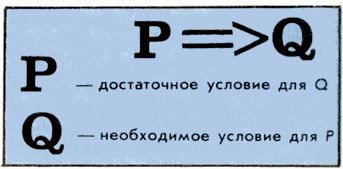
\includegraphics[width=0.5\textwidth]{lectures/files/lec_3_19.09.2025-18-44-35.png}
  \label{fig:lec_3_19.09.2025-18-44-35.png}
\end{figure}

\section{Комбинаторика и Бином Ньютона}
\subsection{Бином Ньютона}

$$ \fbox{
    $ (a + b)^n = \Sum{k = 0}{n} C^k_n a^k b^{n-k} $
} $$

$$ C^0_n a^0 b^{n - 0} + C^1_n a^1 b^{n - 1} + \ldots + C^n_n a^n b^{n - n} $$

где $C^0_n, C^1_n, \ldots $ - биномиальные коэффициенты

\subsection{Комбинаторика}

\begin{definition}
    \textbf{Перестановка} - упорядоченное множество размера $n$ 

    \# перестановок $= n!$
\end{definition}

\begin{definition}
    \textbf{Размещения} - упорядоченное подмножество размера $k$ множества размера $n$

    \# размещений $= \frac{n!}{(n - k)!} = A^k_n$
\end{definition}

\begin{definition}
    \textbf{Сочетания} - неупорядоченное подмножество размера $k$ множества размера $n$

    Одному сочетанию соответствуют $k!$ размещений

    $ \frac{A^k_n}{k!} = \frac{n!}{k!(n-k)!} = C^k_n $
\end{definition}

\section{Последовательности}

\begin{definition}
    \textbf{Последовательность} - индексированный набор чисел

    $ \{a_n\}_{n \in \N} $
\end{definition}

\subsection{Способы задания последовательности}
\begin{itemize}
    \item[1)] Формульный $a_n = n^2 + n - 7$
    \item[2)] Рекуррентный $a_1 = 1, a_2 = 1, a_n = a_{n-1} + a_{n-2} $
\end{itemize}

\begin{definition}
    Последовательность называется \textbf{ограниченной}, если
    $$ \fbox{
        $ \exists c\ \forall n\ |a_n| \leq c $
    } = P(\{a_n\}) $$
    И \textbf{неограниченной}, если
    $$ \fbox{
        $ \forall c\ \exists n(c)\ |a_{n(c)}| > c $
    } $$
\end{definition}

\begin{example}
    $$ a_n = \frac{3n^2 + 5n - 2}{2n^2 + n + 1} $$
    $$ \l|\frac{3n^2 + 5n - 2}{2n^2 + n + 1}\r| \leq \l|\frac{3n^2 + 5n^2}{2n^2}\r| \leq \l|\frac{8n^2}{2n^2}\r| \leq c $$
    $$ 4 \leq c $$
    $$ \exists c = \pi^2\ \forall n\ \l|\frac{3n^2 + 5n - 2}{2n^2 + n + 1}\r| \leq c$$
\end{example}

\subsection{Предел последовательности}

\begin{definition}
    Окрестность точки $A$: $U_{\eps}(A) = (A - \eps; A + \eps)$
\end{definition}

\begin{figure}[h]
  \centering
  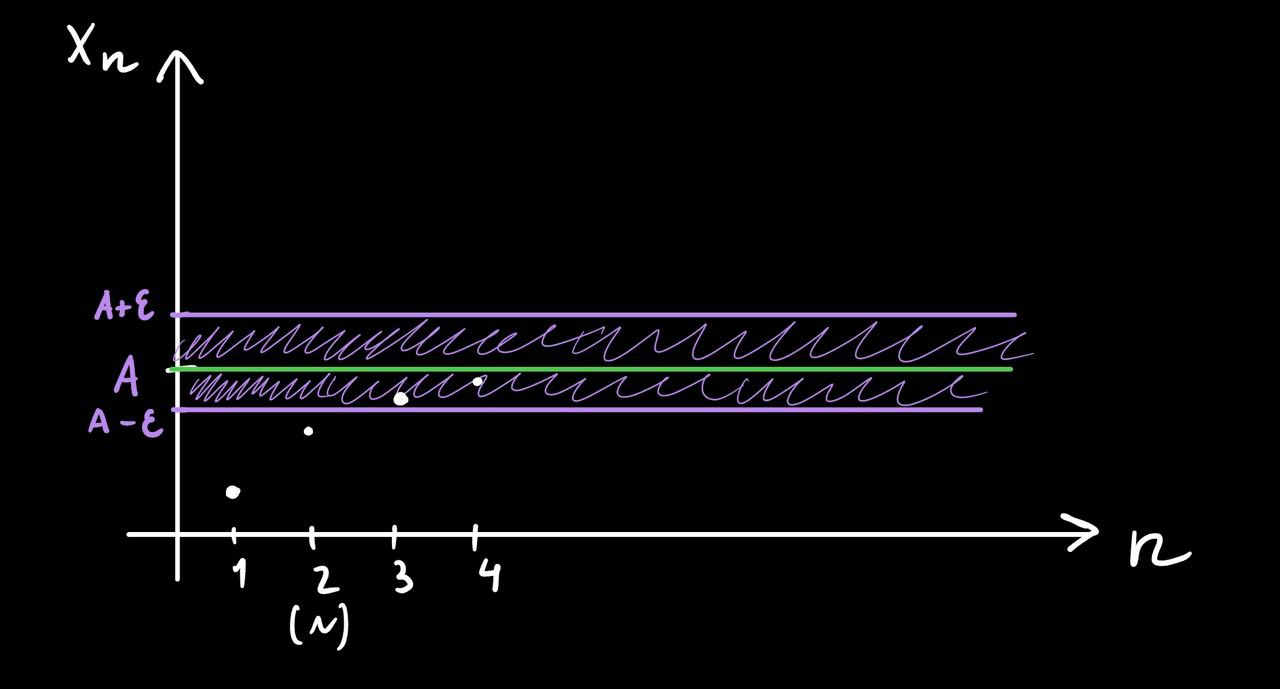
\includegraphics[width=0.8\textwidth]{lectures/files/lec_3_19.09.2025-13-56-05.png}
  \label{fig:lec_3_19.09.2025-13-56-05.png}
\end{figure}

\begin{definition}
    $\Lim{n}{\infty} a_n = A$, если 
    $$\fbox{$ \forall \eps > 0\ \exists N \in \N\ \forall n > N\ |a_n - A| < \eps $}$$
    $$ \Updownarrow $$
    $$ \forall \eps > 0\ \exists N \in \N\ \forall n > N\ -\eps < a_n - A < \eps $$
    $$ \Updownarrow $$
    $$ \forall \eps > 0\ \exists N \in \N\ \forall n > N\ A-\eps < a_n < A+\eps $$
    $$ \Updownarrow $$
    $$ \forall \eps > 0\ \exists N \in \N\ \forall n > N\ a_n \in U_\eps(A) $$
\end{definition}

\begin{example}
    Доказать, что
    $ \Lim{n}{\infty} \frac{1}{n} = 0 $

    $$ \forall \eps > 0\ \exists N \in \N\ \forall n > N\ \l|\frac{1}{n} - 0\r| < \eps $$
    $$ \frac{1}{n} < \eps $$
    $$ n > \frac{1}{\eps} $$
    $$ N(\eps) = \l\lceil \frac{1}{\eps} + 1 \r\rceil $$
\end{example}

\begin{definition}
    Последовательность называется \textbf{сходящейся}, если у нее есть предел 
    $$ \Updownarrow $$
    $$ \exists a : \Lim{n}{\infty} a_n = A $$
\end{definition}

\newpage

\subsection{Теорема об ограниченности сходящейся последовательности}
\begin{theorem}
    Если последовательность сходящаяся, то она ограничена
\end{theorem}
\begin{Proof}
    Рассмотрим $\{a_n\}$
    $$ \exists A\ \forall \eps > 0\ \exists N \in \N\ \forall n > N\ |a_n - A| < \eps $$
    $$ \exists A\ \exists N(1) \in \N\ \forall n > N(1)\ |a_n - A| < 1 \Leftrightarrow a_n \in U_1(A) $$
    Очевидно, что элементов $a_k,\ $где $ k <= N(1)$ конечное число. А для всех элементов $a_n,\ n > N(1)$ выполняется $|a_n - A| < 1$. Тогда можем взять нижнюю границу $min\{a_1,\ldots,a_{N(1)}, A-1\}$ и верхнюю $max\{a_1,\ldots,a_{N(1)}, A+1\}$.
\end{Proof}

\begin{figure}[h]
  \centering
  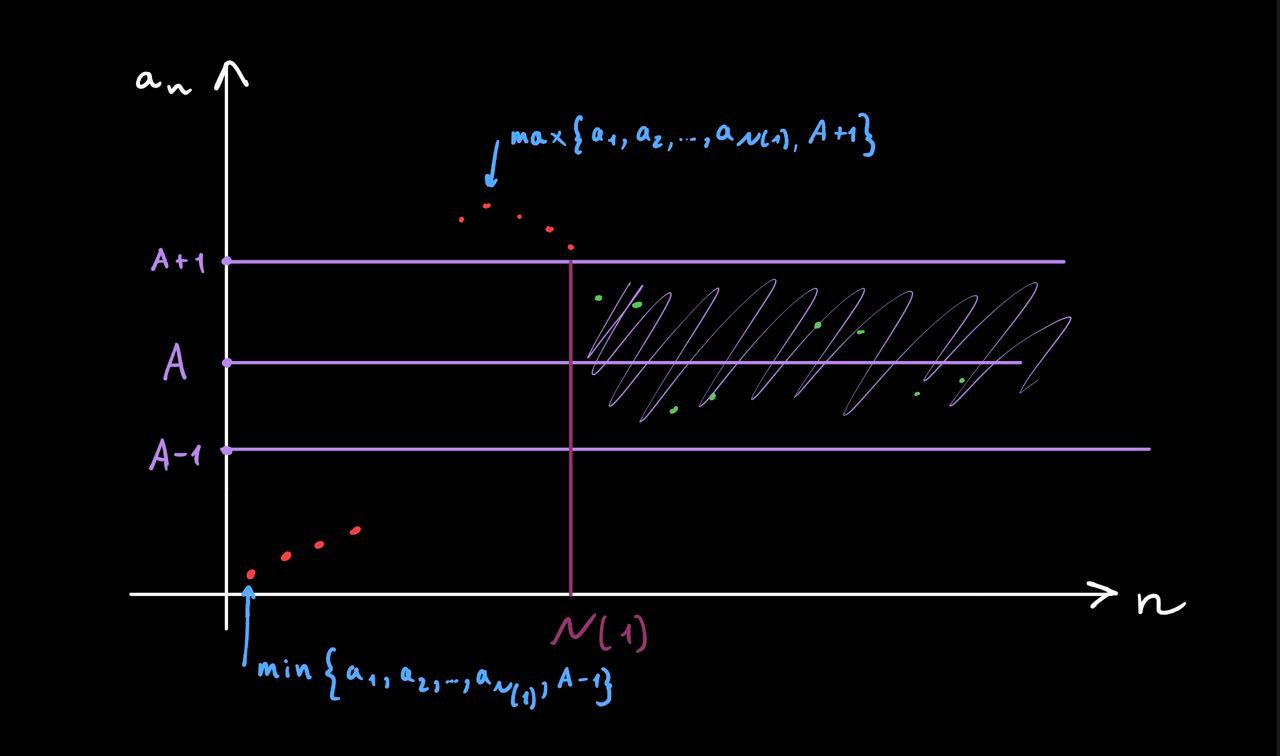
\includegraphics[width=0.8\textwidth]{lectures/files/lec_3_19.09.2025-14-15-52.png}
  \caption{К доказательству}
  \label{fig:lec_3_19.09.2025-14-15-52.png}
\end{figure}

\begin{theorem}
    У последовательности может быть только 1 предел
\end{theorem}

\begin{Proof}
    Пп $\exists$ хотя бы 2 lim : $A$ и $B$, $A \neq B$
    $$ \forall \eps > 0\ \exists N_1(\eps) \in \N\ \forall n > N_1(\eps)\ a_n \in U_{\eps}(A) $$
    $$ \forall \eps > 0\ \exists N_2(\eps) \in \N\ \forall n > N_2(\eps)\ a_n \in U_{\eps}(B) $$
    Возьмем $\eps_0 = \frac{|A - B|}{3}$ и $n_0 = N_1(\eps_0) + N_2(\eps_0) $

    Получаем
    $$ a_{n_0} \in U_{\eps_0}(A),\ a_{n_0} \in U_{\eps_0}(B) $$
    Но 
    $$ U_{\eps_0}(A) \cap U_{\eps_0}(B) = \varnothing $$
    Противоречие
\end{Proof}

\subsection{Арифметика предела}
$ \Lim{n}{\infty}a_n = A $, $ \Lim{n}{\infty}b_n = B $, то

\begin{itemize}
    \item[1)] $\Lim{n}{\infty}(a_n + b_n) = A + B$
    \item[2)] $\Lim{n}{\infty}(a_n \cdot b_n) = A \cdot B$
    \item[3)] $\Lim{n}{\infty}\frac{a_n}{b_n} = \frac{A}{B}$ $(b_n \neq 0; B \neq 0)$
    \item[4)] $\Lim{n}{\infty}\sqrt{a_n} = \sqrt{A}$ $(a_n \geq 0; A \geq 0)$
\end{itemize}

\begin{Proof}[Доказательство свойства 1]
    $$ \forall \eps > 0\ \exists N_1(\eps) \in \N\ \forall n > N_1(\eps)\ |a_n - A| < \eps $$
    $$ \forall \eps > 0\ \exists N_2(\eps) \in \N\ \forall n > N_2(\eps)\ |b_n - B| < \eps $$
    Хотим
    $$ \forall \eps > 0\ \exists N_3(\eps) \in \N\ \forall n > N_3(\eps)\ |(a_n + b_n) - (A + B)| < \eps $$
    $$\Updownarrow$$
    $$ \forall \eps > 0\ \exists N_3(\eps) \in \N\ \forall n > N_3(\eps)\ |(a_n - A) + (b_n - B)| < \eps $$
    $$\Uparrow$$
    $$ \forall \eps > 0\ \exists N_3(\eps) \in \N\ \forall n > N_3(\eps)\ \underbrace{|a_n - A|}_{< \frac{\eps}{3}} + \underbrace{|b_n - B|}_{< \frac{2\eps}{3}} < \eps $$
    $$ \forall n > N_1\l(\frac{\eps}{3}\r)\ \forall n > N_2\l(\frac{2\eps}{3}\r)$$
    $$ N_3(\eps) = max\l\{N_1\l(\frac{\eps}{3}\r), N_2\l(\frac{2\eps}{3}\r)\r\}$$
\end{Proof}

Примечание: Доказательства свойств 2 и 3, рассмотренные далее, были выведены после доказательства теоремы о произведении б.м. и огр. последовательностей

\begin{Proof}[Доказательство свойства 2]
    Хотим
    $$\Lim{n}{\infty}(a_n \cdot b_n) = A \cdot B$$
    По теореме о связи предела с бесконечно малой последовательностью
    $$ \alpha_n=(a_n - A) \text{ --- б.м.} ,\ \beta_n=(b_n - B) \text{ --- б.м.} $$
    Хотим
    $$ (a_n b_n - AB) \text{~--- б.м.} $$
    $$ (a_n b_n - AB) = (\alpha_n + A)(\beta_n + B) - AB = \alpha_n\beta_n + \alpha_nB + A\beta_n + AB - AB = $$
    $$ =\underbrace{\alpha_n\beta_n}_{\text{б.м.}} + \underbrace{\alpha_nB}_{\text{б.м.}} + \underbrace{\underbrace{A}_{\text{огр}}\underbrace{\beta_n}_{\text{б.м.}}}_{\text{б.м.}} = \text{б.м.} + \text{б.м.} + \text{б.м.} = \text{б.м.}$$
\end{Proof}

\begin{Proof}[Доказательство свойства 3]
    Хотим 
    $$\Lim{n}{\infty}\frac{a_n}{b_n} = \frac{A}{B}\ (b_n \neq 0; B \neq 0)$$
    По теореме о связи предела с бесконечно малой последовательностью
    $$ \alpha_n=(a_n - A) \text{ --- б.м.} ,\ \beta_n=(b_n - B) \text{ --- б.м.} $$
    Хотим
    $$ \frac{a_n}{b_n} - \frac{A}{B} \text{ --- б.м.} $$
    $$ \frac{a_n}{b_n} - \frac{A}{B} = \frac{\alpha_n + A}{\beta_n + B} - \frac{A}{B} = \frac{(\alpha_n + A)B - A(\beta_n + B)}{(\beta_n + B)B} = $$
    $$ = \frac{(\alpha_n + A)B - A(\beta_n + B)}{(\beta_n + B)B} = \frac{\alpha_nB + AB - A\beta_n - AB}{b_nB} = \frac{\alpha_nB - A\beta_n}{b_nB} = $$
    $$ = \underbrace{\frac{1}{b_n} \cdot \frac{1}{B}}_{\text{огр $\cdot$ огр}} \cdot \underbrace{(\alpha_nB - A\beta_n)}_{\text{б.м}} = \text{б.м.} $$

\end{Proof}

\subsection{Бесконечно большая и бесконечно малая последовательности}

\begin{definition}
    \textbf{Бесконечно малой} (б.м.) последовательностью называют последовательность $\{a_n\}_{n\in\N}$ такую что, $ \Lim{n}{\infty} a_n = 0 $
\end{definition}

\begin{definition}
    \textbf{Бесконечно большой} (б.б.) последовательностью называют последовательность $\{b_n\}_{n\in\N}$ такую что, $ \Lim{n}{\infty} b_n = \infty $

    $$ \forall M > 0\ \exists N(M) \in \N\ \forall n > N(M)\ |b_n| > M $$
    $$ b_n > M\ (+ \infty) $$
    $$ b_n < M\ (- \infty) $$
\end{definition}

\begin{theorem}
    $$\frac{1}{\text{б.б.}} = \text{б.м.}$$
\end{theorem}

\begin{Proof}
    Пусть $b_n$ - б.б. Тогда
    $$ \forall M > 0\ \exists N_1(M) \in \N\ \forall n > N_1(M)\ |b_n| > M $$
    Хотим $a_n = \frac{1}{b_n}$ - б.м.:
    $$ \forall \eps > 0\ \exists N_2(\eps)\ \forall n > N_2(\eps)\ |a_n| < \eps $$
    $$ \l|\frac{1}{b_n}\r| < \eps $$
    $$ \l|b_n\r| > \frac{1}{\eps} $$
    Возьмем $N_2(\eps) = N_1\l(\frac{1}{\eps}\r) + 1$
\end{Proof}

\begin{theorem}
    \center{б.м. $\cdot$ огр. = б.м.}
\end{theorem}

\begin{Proof}
    Хотим $ a_n \cdot b_n = c_n $, где $a_n, c_n$ - б.м., $b_n$ - огр.

    $$ \forall \eps > 0\ \exists N_1(\eps) \in \N\ \forall n > N_1(\eps)\ |a_n| < \eps $$
    $$ \exists c\ \forall n \in \N\ |b_n| \leq c $$
    Хотим:
    $$ \forall \eps > 0\ \exists N_2(\eps) \in \N\ \forall n > N_2(\eps)\ |a_n \cdot b_n| < \eps $$
    $$ \Uparrow $$
    $$ |a_n| \cdot |b_n| < \eps $$
    $$ |a_n| \cdot c < \eps $$
    $$ |a_n| < \frac{\eps}{c} $$

    Возьмем $N_2(\eps) = N_1\l(\frac{\eps}{c}\r)$
\end{Proof}

\begin{example}
    б.б. + б.б.

    Мы точно не можем сказать, чем будет являться эта сумма. Например $n + (-n) = 0$ и $n + n = 2n$
\end{example}

\begin{example}
    б.б. + огр. = б.б.

    Покажем, что это так

    Хотим: $b_n + c_n = u_n$ соответственно. Тогда:
    $$ \forall M > 0\ \exists N(M) \in \N\ \forall n > N(M)\ |b_n| > M $$
    $$ \exists C > 0\ \forall n \in \N\ |c_n| \leq C $$

    Хотим:
    $$ \forall K > 0\ \exists N_2(K) \in \N\ \forall n > N_2(K)\ |b_n + c_n| > K $$
    Так, как $ |x + y| \geq |x| - |y| $:
    $$ |b_n| - |c_n| > K $$
    $$ |b_n| - C > K $$
    $$ |b_n| > K + C $$
    Возьмем $N_2(K) = N(K + C)$
\end{example}

\begin{theorem}
    $$ \Lim{n}{\infty} a_n = A \Leftrightarrow (a_n - A) = \alpha_n \text{ - бесконечно малая} $$
\end{theorem}

\begin{Proof}
    $$ \forall \eps > 0\ \exists N_1(\eps) \in \N\ \forall n > N_1(\eps)\ |a_n - A| < \eps $$
    Хотим
    $$ \forall \eps > 0\ \exists N_2(\eps) \in \N\ \forall n > N_2(\eps)\ |(a_n - A) - 0| < \eps $$
    $$ N_2(\eps) = N_1(\eps) $$
\end{Proof}

\begin{remark}
    Теперь можно спокойно доказать свойство 2) из арифметики пределов
\end{remark}

\begin{remark}
    Произведение бесконечно малых - бесконечно малая последовательность. Так как можно представить одну из них как ограниченную и использовать теорему выше
\end{remark}

\begin{definition}
    Назовем последовательность $d_n$ \textbf{отделимой от нуля}, если:
    $$ \exists \delta > 0\ \forall n \in \N\ |d_n| \geq \delta $$
\end{definition}

\begin{example}
    $(-1)^n$
\end{example}

\begin{theorem}
    $$ \frac{1}{\text{огр}} = \text{отделима от нуля},\ \frac{1}{\text{отделима от нуля}} = \text{огр} $$
\end{theorem}

\begin{Proof}
    $$ \exists \delta > 0\ \forall n \in \N\ |d_n| \geq \delta $$
    $$ u_n = \frac{1}{d_n},\ \exists c > 0\ \forall n \in \N\ |u_n| \leq c $$
    $$ \Updownarrow $$
    $$ \l|\frac{1}{d_n}\r| \leq c $$
    $$ \Updownarrow $$
    $$ |d_n| \geq \frac{1}{c} $$
    Возьмем $ c = \frac{1}{\delta} $. Тогда $ |d_n| \geq \delta $ верно $ \forall n \in \N $
\end{Proof}

\begin{theorem}
    Если $ \Lim{n}{\infty} u_n = U;\ u_n, U \neq 0$,\ то $u_n$ отделима от нуля
\end{theorem}

\begin{Proof}
    $$ \forall \eps > 0\ \exists N(\eps) \in \N\ \forall n > N(\eps)\ |u_n - U| < \eps $$
    Хотим
    $$ \exists \delta > 0\ \forall n \in \N\ |u_n| \geq \delta $$
    Возьмем $ \eps_0 = \frac{|U|}{2} $
    $$ \exists N_0 = N\l(\frac{|U|}{2}\r) = N(\eps_0) $$
    $$ \forall n > N_0\ u_n \in U_{\frac{|U|}{2}}(U) $$
    Очевидно, что существует конечное число $u_k,\ k \leq N(\eps_0)$, причем $u_k \neq 0$

    Возьмем $\delta = min\{|u_1|, |u_2|, \ldots, \frac{|U|}{2}\}$
\end{Proof}

\subsection{Предельный переход в неравенствах}

\begin{theorem}
    Если $\exists N_0\ \forall n > N_0\ a_n > b_n$ и $a_n \underset{n \to \infty}{\to} A$ и $b_n \underset{n \to \infty}{\to} B$, то 
    $ A \geq B $
\end{theorem}

\begin{Proof}
    Пп $A < B$. Возьмем $\eps_0 = \frac{B - A}{2} $
    $$ \exists N_1(\eps_0)\ \forall n > N_1(\eps_0)\ a_n \in U_{\eps_0}(A) $$
    $$ \exists N_2(\eps_0)\ \forall n > N_2(\eps_0)\ b_n \in U_{\eps_0}(B) $$
    Возьмем $n_0 = N_1(\eps_0) + N_2(\eps_0) + N_0$
    Тогда по условию $a_{n_0} > b_{n_0}$, но также $a_{n_0} < b_{n_0}$ (так как окрестность $a$ по предположению левее окрестности $b$). Получили противоречие
\end{Proof}

\subsection{Теорема о зажатой последовательности}
\begin{theorem}[Теорема о зажатой последовательности]
    Если $\exists N_0\ \forall n > N_0\ a_n \leq c_n \leq d_n$, а также $a_n \underset{n \to \infty}{\to} A$ и $d_n \underset{n \to \infty}{\to} A$, то $c_n \underset{n \to \infty}{\to} A$
\end{theorem}

\begin{Proof}
    $$a_n \underset{n \to \infty}{\to} A;\ \forall \eps > 0\ \exists N_1(\eps)\ \forall n > N_1(\eps)\ A-\eps < a_n < A+\eps$$
    $$d_n \underset{n \to \infty}{\to} A;\ \forall \eps > 0\ \exists N_2(\eps)\ \forall n > N_2(\eps)\ A-\eps < d_n < A+\eps$$
    Хотим
    $$c_n \underset{n \to \infty}{\to} A;\ \forall \eps > 0\ \exists N_3(\eps)\ \forall n > N_3(\eps)\ A-\eps < c_n < A+\eps$$
    Получаем
    $$ \underbrace{A-\eps <}_{\forall n > N_1(\eps)} a_n \underbrace{\leq c_n \leq}_{\forall n > N_0} d_n \underbrace{< A+\eps}_{\forall n > N_2(\eps)} $$
    Возьмем $N_3(\eps) = max\{N_1(\eps),\ N_2(\eps),\ N_0\}$
\end{Proof}

\section{Действительные числа}

\begin{definition}
    Множество \textbf{действительных чисел} - это четверка $(\R; +; \times; \leq)$ (множество, 2 операции, 1~отношение)
\end{definition}

\begin{remark}
    Отличие операции от отношения. Для того чтобы задать операцию, нужно поставить в соответствие для каждой пары чисел число $(\R \times \R \to \R)$. В отношении для каждой пары чисел нужно поставить в соответствие 0 или 1 $(\R \times \R \to \{0, 1\})$.
\end{remark}

\subsection{Аксиома непрерывности}
$ A, B \subset \R $
\begin{itemize}
    \item[1)] $ A, B \neq \varnothing $
    \item[2)] $ \forall x \in A\ \forall y \in B\ x \leq y$
\end{itemize}
Тогда $ \exists \xi \in \R : \forall x \in A\ \forall y \in B\ x \leq \xi \leq y $

\begin{definition}
    \textbf{Верхней гранью} множества $A \subset \R$ называется число $C \in \R$, такое что $\forall x \in A\ x \leq C$
\end{definition}

\begin{definition}
    \textbf{Точной верхней гранью} $(sup\ A)$ ограниченного сверху множества $A$ называют наименьшую верхнюю грань множества $A$
\end{definition}

\begin{definition}
    \textbf{Нижней гранью} множества $A \subset \R$ называется число $D \in \R$, такое что $\forall x \in A\ x \geq D$
\end{definition}

\begin{definition}
    \textbf{Точной нижней гранью} $(inf\ A)$ ограниченного снизу множества $A$ называют наибольшую нижнюю грань множества $A$
\end{definition}

\begin{example}
    $A = (-1; 0)$. Множество верхних граней: $[0; +\infty),\ sup\ A = 0$
\end{example}

\begin{theorem}
    У ограниченного сверху множества есть точная верхняя грань
\end{theorem}

\begin{Proof}
    \[\begin{array}{l}
        \l.
        \begin{array}{l}
            A - \text{огр. сверху},\ A \neq \varnothing\\
            B = \{\text{верхние грани A}\},\ B \neq \varnothing\\
            \forall x \in A\ \forall y \in B\ x \leq y\\
        \end{array}
        \r]
        \l.
        \exists \xi \in \R: \forall x \in A\ \forall y \in B\ x \leq \xi \leq y
        \r.
    \end{array}\]
    \begin{itemize}
        \item[1)] Из $x \leq \xi$ получаем, что $\xi$ - верхняя грань $A \Rightarrow \xi \in B$
        \item[2)] Так, как $\xi \leq y$, то $\xi$ - минимальный элемент из $B$. \fbox{$\xi = sup\ A$}
    \end{itemize}
\end{Proof}

\begin{definition}
    \textbf{Точной верхней гранью неограниченного сверху множества} назовем $+\infty$
\end{definition}

\subsection{Теорема Вейерштрасса}
\begin{definition}
    $\{a_n\}$ - \textbf{неубывает}, если $a_{n+1} \geq a_n$
\end{definition}

\begin{definition}
    $\{a_n\}$ - \textbf{возрастает}, если $a_{n+1} > a_n$
\end{definition}

\begin{example}[Пример (3-й способ доказательства монотонности)]
    Доказать, что последовательность $a_n = \l(1 + \frac{1}{n}\r)^n$ строго возрастает

    Необходимо доказать: $\forall n\ a_{n+1} > a_n$
    $$1 < \frac{a_{n+1}}{a_n} = \frac{\l(1 + \frac{1}{n+1}\r)^{n+1}}{\l(1 + \frac{1}{n}\r)^n} = \l(\frac{n+2}{n+1}\r)^{n+1} \cdot \l(\frac{n}{n+1}\r)^n =$$
    $$ = \l(\frac{n(n+2)}{(n+1)^2}\r)^n \cdot \l(\frac{n+2}{n+1}\r) $$
    По неравенству Бернулли \fbox{$ \forall n \in \N\ \forall x \geq -1\ (1 + x)^n \geq 1 + xn $}
    $$ \l(\frac{n(n+2)}{(n+1)^2}\r)^n \cdot \l(\frac{n+2}{n+1}\r) = \l(\frac{n^2 + 2n}{n^2 + 2n + 1}\r)^n \cdot \l(\frac{n+2}{n+1}\r) = $$
    $$ = \l(1 + \underbrace{\l(- \frac{1}{(n + 1)^2}\r)}_{\geq -1}\r)^n \cdot \l(\frac{n+2}{n+1}\r) \geq \l(1 - \frac{n}{(n + 1)^2}\r) \cdot \l(\frac{n+2}{n+1}\r) = $$
    $$ = \frac{(n^2 + n + 1)(n + 2)}{(n+1)^3} = \frac{n^3 + 3n^2 + 3n + 2}{n^3 + 3n^2 + 3n + 1} > 1 $$
\end{example}

\begin{theorem}[Теорема Вейерштрасса]
    Если $\{a_n\}$ неубывает и ограничена сверху, то она сходится
\end{theorem}

\begin{Proof}
    $ \{a_n\} = A \neq \varnothing \text{, огр. сверху} $

    $ \exists sup\ A = a \in \R $

    Хотим доказать: $a_n \underset{n \to \infty}{\to} A $

    $$ \forall \eps > 0\ \exists N(\eps)\ \forall n > N(\eps)\ \underbrace{|a_n - A|}_{\leq 0} < \eps $$
    $$ A - a_n < \eps $$
    $$ a_n > A - \eps \Leftrightarrow a_{N(\eps) + 1} > A - \eps$$

    Тогда докажем:
    $$ \forall \eps > 0\ \exists N(\eps) \in \N\ a_{N(\eps) + 1} > A - \eps $$

    Пп 
    $$ \exists \eps_0 > 0\ \forall N \in \N\ a_{N+1} \leq A - \eps_0 $$
    $$ \Updownarrow $$
    $$ \exists \eps_0 > 0\ \forall n \in \N\ a_{n} \leq A - \eps_0 $$
    Получаем, что самая маленькая верхняя граница $ = A - \eps_0 $, но $ sup\ a_n = A$. $\bot$
\end{Proof}

\textbf{Контрпример} (Если $\{a_n\}$ сходится, то необязательно она неубывает)

$$ \fbox{
    $ a_n = \frac{\sin n}{2^n} \underset{n \rightarrow \infty}{\rightarrow} 0 $
} $$
\begin{theorem}
    $$ \exists \Lim{n}{\infty} \l(1 + \frac{1}{n}\r)^n = e $$
\end{theorem}

\begin{Proof}
    Ранее мы доказали, что данная последовательность неубывает.
    $$ \l(1 + \frac{1}{n}\r)^n = \l(\frac{1}{n} + 1\r)^n = \Sum{k = 0}{n} \ C^k_n \l(\frac{1}{n}\r)^k 1^{n-k} =$$
    $$ = 1 + \frac{n!}{(n-1)!\ 1!} \cdot \frac{1}{n} + \ldots + \frac{n!}{(n-k)!\ k!} \cdot \frac{1}{n^k} + \ldots = $$
    $$ = 1 + 1 + \ldots + \underbrace{\frac{n}{n}}_{\leq 1} \cdot \underbrace{\frac{n-1}{n}}_{\leq 1} \cdot \ldots \cdot \underbrace{\frac{n - k + 1}{n}}_{\leq 1} \cdot \frac{1}{k!} + \ldots < 1 + 1 + \frac{1}{2!} + \ldots + \frac{1}{n!} $$

    Напоминение о телескопических суммах:
    $$
    \boxed{
    \begin{aligned}
        \Sum{k=1}{n} \frac{1}{k(k+1)} = \Sum{k=1}{n} \l(\frac{1}{k} - \frac{1}{k+1} \r) = 1 - \frac{1}{n+1}
    \end{aligned}
    }$$

    Хотим получить нечто похожее, тогда выкинем из каждого знаменателя все множители, кроме последних двух:
    $$ 1 + 1 + \frac{1}{2!} + \ldots + \frac{1}{n!} \underbrace{<}_{n \geq 4} 2 + \frac{1}{1 \cdot 2} + \frac{1}{2 \cdot 3} + \ldots + \frac{1}{(n - 1) \cdot n} = 2 + \l(1 - \frac{1}{n} \r) < 3 $$
\end{Proof}

\subsection{Предел рекуррентно заданных последовательностей}
\subsection{Постоянная Эйлера}

\section{Подпоследовательности}

\begin{definition}
    \textbf{Подпоследовательностью} последовательности $\{a_n\}$ называется последовательность $\{b_k\}$, такая что $b_k = a_{n_k}$, где $n_k$ - строго возрастающая последовательность номеров ($\N$)
\end{definition}

\begin{remark}[Замечание]
    $$ n_k \geq k $$
\end{remark}

\begin{example}
    $ a_n = \sin \frac{\pi n}{2} $

    $ b_k = a_{4k} = \sin 2\pi k \equiv 0$

    $ c_k = a_{4k - 1} = \sin \frac{\pi (4k - 1)}{2} \equiv -1$

    $ d_k = a_{2k + 1} = \sin \frac{\pi (2k + 1)}{2} = (-1)^k  $
\end{example}

\subsection{Частичные пределы}
\subsection{Предельные точки} 
\subsection{Свойства частичных пределов}
\newpage
\subsection{Теорема Больцано-Вейерштрасса}

\begin{theorem}
Если $a_n \underset{n \to \infty}{\to} A, \text{ то}\ \forall n_k\ b_k = a_{n_k} \underset{n \to \infty}{\to} A $ 
\end{theorem}

\begin{Proof}
    $$ \forall \eps > 0\ \exists N(\eps)\ \forall n > N(\eps)\ |a_n - A| < \eps $$
    Хотим
    $$ \forall \eps > 0\ \exists K(\eps)\ \forall k > k(\eps)\ |a_{n_k} - A| < \eps $$
    Возьмем $K(\eps) = N(\eps)$
    \[\begin{array}{l}
        \l.
        \begin{array}{l}
            \forall k > N(\eps)\\
            \text{т.к } n_k \geq k
        \end{array}
        \r]
        \l. \Rightarrow \r.
        \l.
        n_k > N(\eps). \text{ Тогда } |a_{n_k} - A| < \eps \text{ истина}
        \r.
    \end{array}\]
\end{Proof}

\begin{figure}[h]
  \centering
  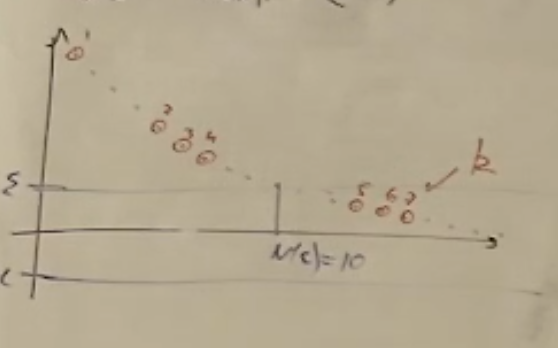
\includegraphics[width=0.5\textwidth]{lectures/files/lec_6_10.10.2025-19-24-42.png}
  \caption{К теореме}
  \label{fig:lec_6_10.10.2025-19-24-42.png}
\end{figure}

\begin{theorem}[Теорема Больцано-Вейерштрасса]
    Если последовательность ограничена, то у нее есть сходящаяся подпоследовательность
\end{theorem}

\subsection{Критерий Коши}

\section{Функции}
\subsection{Функция. График функции}
\subsection{Инъекция, сюрьекция, биекция} 
\subsection{Обратимость функции}
\subsection{Предел функции по Коши}
\subsection{Предел функции по Гейне}

% AUTO-LECTURES
\end{document}
